\documentclass{article} 
\usepackage{graphicx}
\title{Bailando Differentiator} 
\author{Dmit} 
\date{December 2023} 
\begin{document} 
\maketitle 
\section{Bailando-Differentiating Func} 
Si senor efectos especiales ye ye ye: $sin(x)$  \newline Si senor una tentacion ye ye ye: $x$ Tu y yo a la fiesta: $1$  \newline Tu y yo toda la noche: $cos(x)*1$  \newline \newline Optimization bailnado: \newline Tu y yo a la fiesta: $cos(x)$  \newline Tu y yo: $cos(x)$  \newline \begin{figure}
\centering
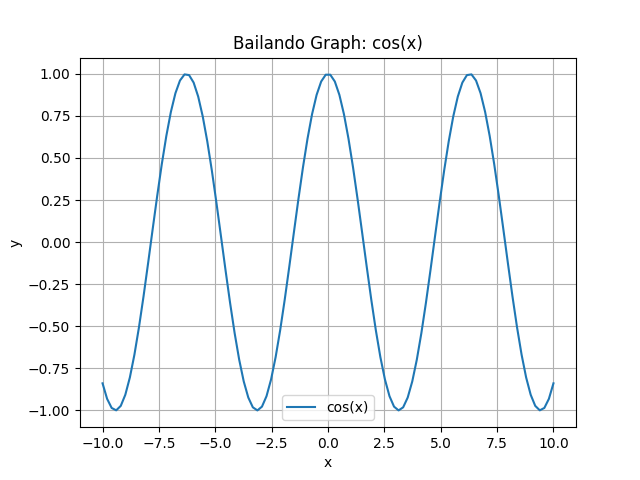
\includegraphics[width=0.8\linewidth]{Bailando Graph.png}
\caption{Bailando: Graph}
\label{fig:my_image}
\end{figure}
Bailando bailando amigos adios: $cos(x)$  \newline adios el silencio loco: $x$ Bailando bailando amigos adios: $1$  \newline adios el silencio loco: $sin(x)*-1*1$ Si senor corona de cristales ye ye ye: $cos(x)$  \newline Si senor una emocion ye ye ye: $x$ Tu y yo a la fiesta: $1$  \newline Tu y yo toda la noche: $sin(x)*-1*1$ Tu y yo a la fiesta: $sin(x)*-1*1$ Tu y yo: $1$ Bailando bailando amigos adios: $0$  \newline adios el silencio loco: $sin(x)*-1$ Bailando bailando amigos adios: $-1$ adios el silencio loco: $0$  \newline Bailando bailando amigos adios: $sin(x)$  \newline adios el silencio loco: $x$ Bailando bailando amigos adios: $1$  \newline adios el silencio loco: $cos(x)*1$ La luna estaba llena sone sone de un palacio: $cos(x)*1*-1+sin(x)*0$ un paraiso que se llama Paradisio: ${cos(x)*1*-1+sin(x)*0}*1+sin(x)*-1*0$  \newline \newline Optimization bailnado: \newline Bailando bailando amigos adios: $\frac{x^2}{2}*-1+0+\frac{1}{1}$  \newline adios el silencio loco: $\frac{x^2}{2}*-1+1$  \newline Bailando bailando amigos adios: $\frac{x^2}{2}*-1+1$  \newline \begin{figure}
\centering
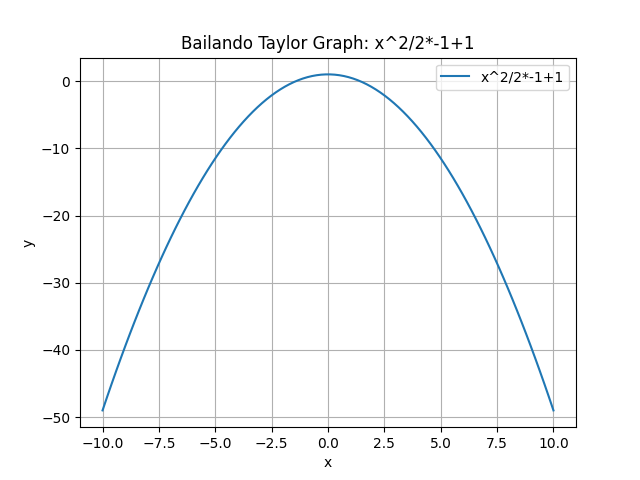
\includegraphics[width=0.8\linewidth]{Bailando Taylor Graph.png}
\caption{Bailando: Taylor Graph}
\label{fig:my_image}
\end{figure}
adios el silencio loco: $cos(x)$  \newline Bailando bailando amigos adios: $x$ adios el silencio loco: $1$  \newline Bailando bailando amigos adios: $sin(x)*-1*1$ adios el silencio loco: $cos(x)$  \newline Bailo sensual: $x$ noche romantica: $1$  \newline melodia: $sin(x)*-1*1$ Si senor efectos especiales ye ye ye: $sin(x)*-1*1$ Si senor una tentacion ye ye ye: $1$ Tu y yo a la fiesta: $0$  \newline Tu y yo toda la noche: $sin(x)*-1$ Tu y yo a la fiesta: $-1$ Tu y yo: $0$  \newline Bailando bailando amigos adios: $sin(x)$  \newline adios el silencio loco: $x$ Bailando bailando amigos adios: $1$  \newline adios el silencio loco: $cos(x)*1$ Si senor corona de cristales ye ye ye: $cos(x)*1*-1+sin(x)*0$ Si senor una emocion ye ye ye: ${cos(x)*1*-1+sin(x)*0}*1+sin(x)*-1*0$  \newline \newline Optimization bailnado: \newline Tu y yo a la fiesta: $cos(x)-\frac{x^2}{2}*-1+0+\frac{1}{1}$  \newline Tu y yo toda la noche: $cos(x)-\frac{x^2}{2}*-1+1$  \newline Tu y yo a la fiesta: $cos(x)-\frac{x^2}{2}*-1+1$  \newline \begin{figure}
\centering
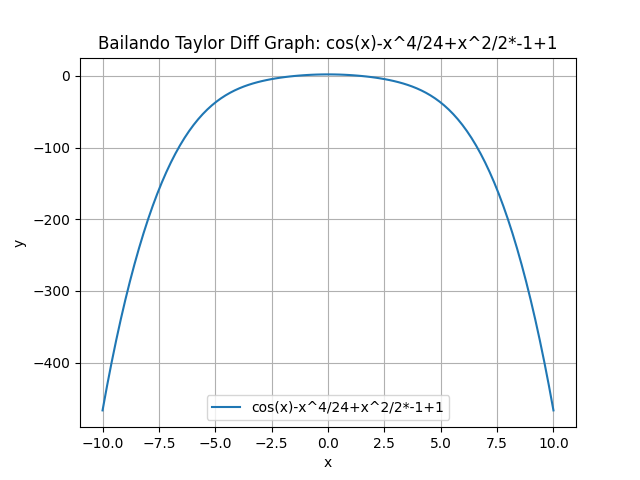
\includegraphics[width=0.8\linewidth]{Bailando Taylor Diff Graph.png}
\caption{Bailando: Taylor Diff Graph}
\label{fig:my_image}
\end{figure}
 \newline \newline Optimization bailnado: \newline Tu y yo: $cos(x)$  \newline 
\end{document}